\chapter{Introducción}

En este capítulo no deben faltar los siguientes apartados:

\section{Motivación del proyecto}

En los últimos años el consumo de energía primaria en España ha aumentado significativamente de unos 88455 ktep($\sim1.03E12 \ kWh$) en 1990 a unos 126107 ktep($\sim 1.43E12 \ kWh$) en 2019, que equivale a un aumento del 42\% respecto a su valor en 1990, llegando a ser su valor máximo unos 146891 ktep($\sim 1.71E12 \ kWh$) en 2007 \cite{libroEnergiaEnEspana2019}.\\\\
De 2008 a 2014, como consecuencia de la crisis económica el consumo energético disminuyó hasta unos 117824 ktep ($\sim 1.37E12 \ kWh$) en 2014, recuperándose a partir del 2015, como se puede observar en la figura \ref{fig:demandaenergiaprimariaproporcion1990}. \\


\begin{figure}[H]
	\centering
	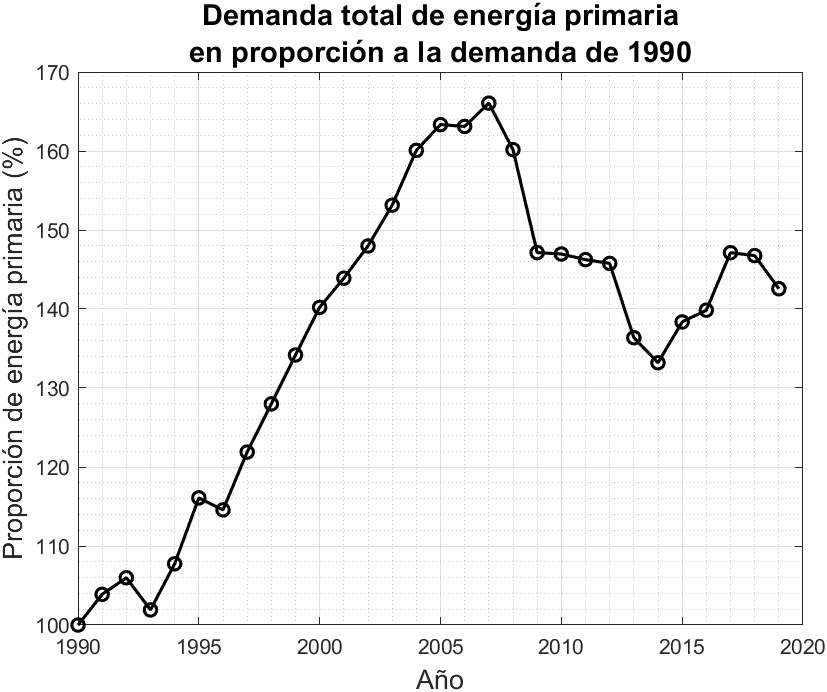
\includegraphics[width=10cm, height=7cm]{figuras/DemandaEnergiaPrimariaProporcion1990}
	\caption[Relación entre demanda total de energía primaria anual]{Representación gráfica de la relación entre la demanda total de energía primaria anual de 1990 hasta 2019 en España. \textit{Fuente obtención de datos: Ministerio para la transición ecológica y el reto demográfico de España.} }
	\label{fig:demandaenergiaprimariaproporcion1990}
\end{figure}
Dicha energía se puede dividir en diferentes categorías según el sector que la consume o la fuente de la misma. En el 2019, un 44.5\% de la energía primaria fue consumida de productos petrolíferos y apenas un 14.5\% de renovables (figura \ref{fig:fuentesenergiasprimarias}), y un 23.6\% de la energía final fue consumida por el sector de la industria (figura \ref{fig:consumoenergiafinalporsectores2019}), representando casi una cuarta parte del consumo total de la energía final en España. Desafortunadamente en todos los procesos energéticos, ya sean de producción, transporte o consumo, una parte de la energía siempre es desaprovechada en forma de calor (conocido como calor residual). Por ejemplo, en 2015 la industria en España consumió aproximadamente 220 TWh de energía, desperdiciándose unos 22 TWh según los cálculos de las estimaciones realizadas en \cite{wasteEnergyindustryEstimate}.

\begin{figure}[H]
	\centering
	\begin{subfigure}[b]{0.48\textwidth}
		\includegraphics[width=\textwidth]{figuras/FuentesEnergíasPrimarias}
		\caption{Consumo de energía por fuente}
		\label{fig:fuentesenergiasprimarias}
	\end{subfigure}
	\hfill
	\begin{subfigure}[b]{0.48\textwidth}
		\centering
		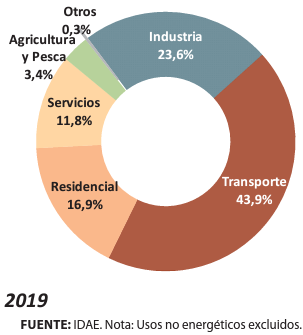
\includegraphics[width=\textwidth]{figuras/consumoEnergiaFinalPorSectores_2019}
		\caption{Consumo de energía por sectores.}
		\label{fig:consumoenergiafinalporsectores2019}
	\end{subfigure}
\caption[Desglose del consumo de energía primaria en España 20]{Desglose del consumo de energía primaria en España 2019 por fuente de energía(\subref{fig:fuentesenergiasprimarias}). Consumo de energía final por sectores en el año 2019 en España(\subref{fig:consumoenergiafinalporsectores2019}). \textit{Fuente:  Ministerio para la transición ecológica y el reto demográfico de España.} }
 \label{fig:consumosEnergiasCategorias}
\end{figure}

Para recuperar esta energía perdida se han desarrollado instalaciones de recuperación de calor residual, no solo para disminuir los costes sino también para disminuir las emisiones de contaminantes, cumpliendo así parte de los objetivos de desarrollo sostenible. El calor residual se puede aprovechar para obtener electricidad o para calentar un fluido para mejorar la eficiencia del mismo u otro proceso, disminuyendo el consumo de combustible o energía.\\

El aprovechamiento del calor residual para el calentamiento de otro fluido se utiliza en la industria. Algunos ejemplos de esto son: los economizadores que se usan en calderas para pre-calentar los fluidos, mejorando el rendimiento térmico, y en el sector residencial se aprovecha el calor obtenido del sistema de enfriamiento de algunos sistemas fotovoltaicos para obtener agua caliente.\\ 

La obtención de electricidad mediante el aprovechamiento del calor residual puede ser por vía de trabajo mecánico o por conversión directa. Por vía de trabajo mecánico se produce mediante ciclos termodinámicos, principalmente el ciclo de Rankine, el cual mediante un intercambiador de calor se genera vapor de agua que luego hace mover unas turbinas que están conectadas a un generador. La conversión directa se basa en la utilización de dispositivos termoeléctricos (\acrshort{teg}), termoiónicos (\acrshort{tic}) y termo-fotovoltaicos (\acrshort{tpv}).\\

La conversión térmica por vías mecánicas es la más conocida y es altamente utilizada, por ejemplo, las centrales nucleares, los sistemas de ciclos combinados, los sistemas de tratamientos de residuos que necesitan ser incinerados(figura \ref{fig:esquemaslomasvalorizacion}), entre otros. También se puede aprovechar el calor residual de la generación eléctrica, como es el caso de los cogeneradores.

%% IMAGENES DE SISTEMAS DE APROVECHAMIENTOS MECÁNICOS
\begin{figure}[H]
	\centering
	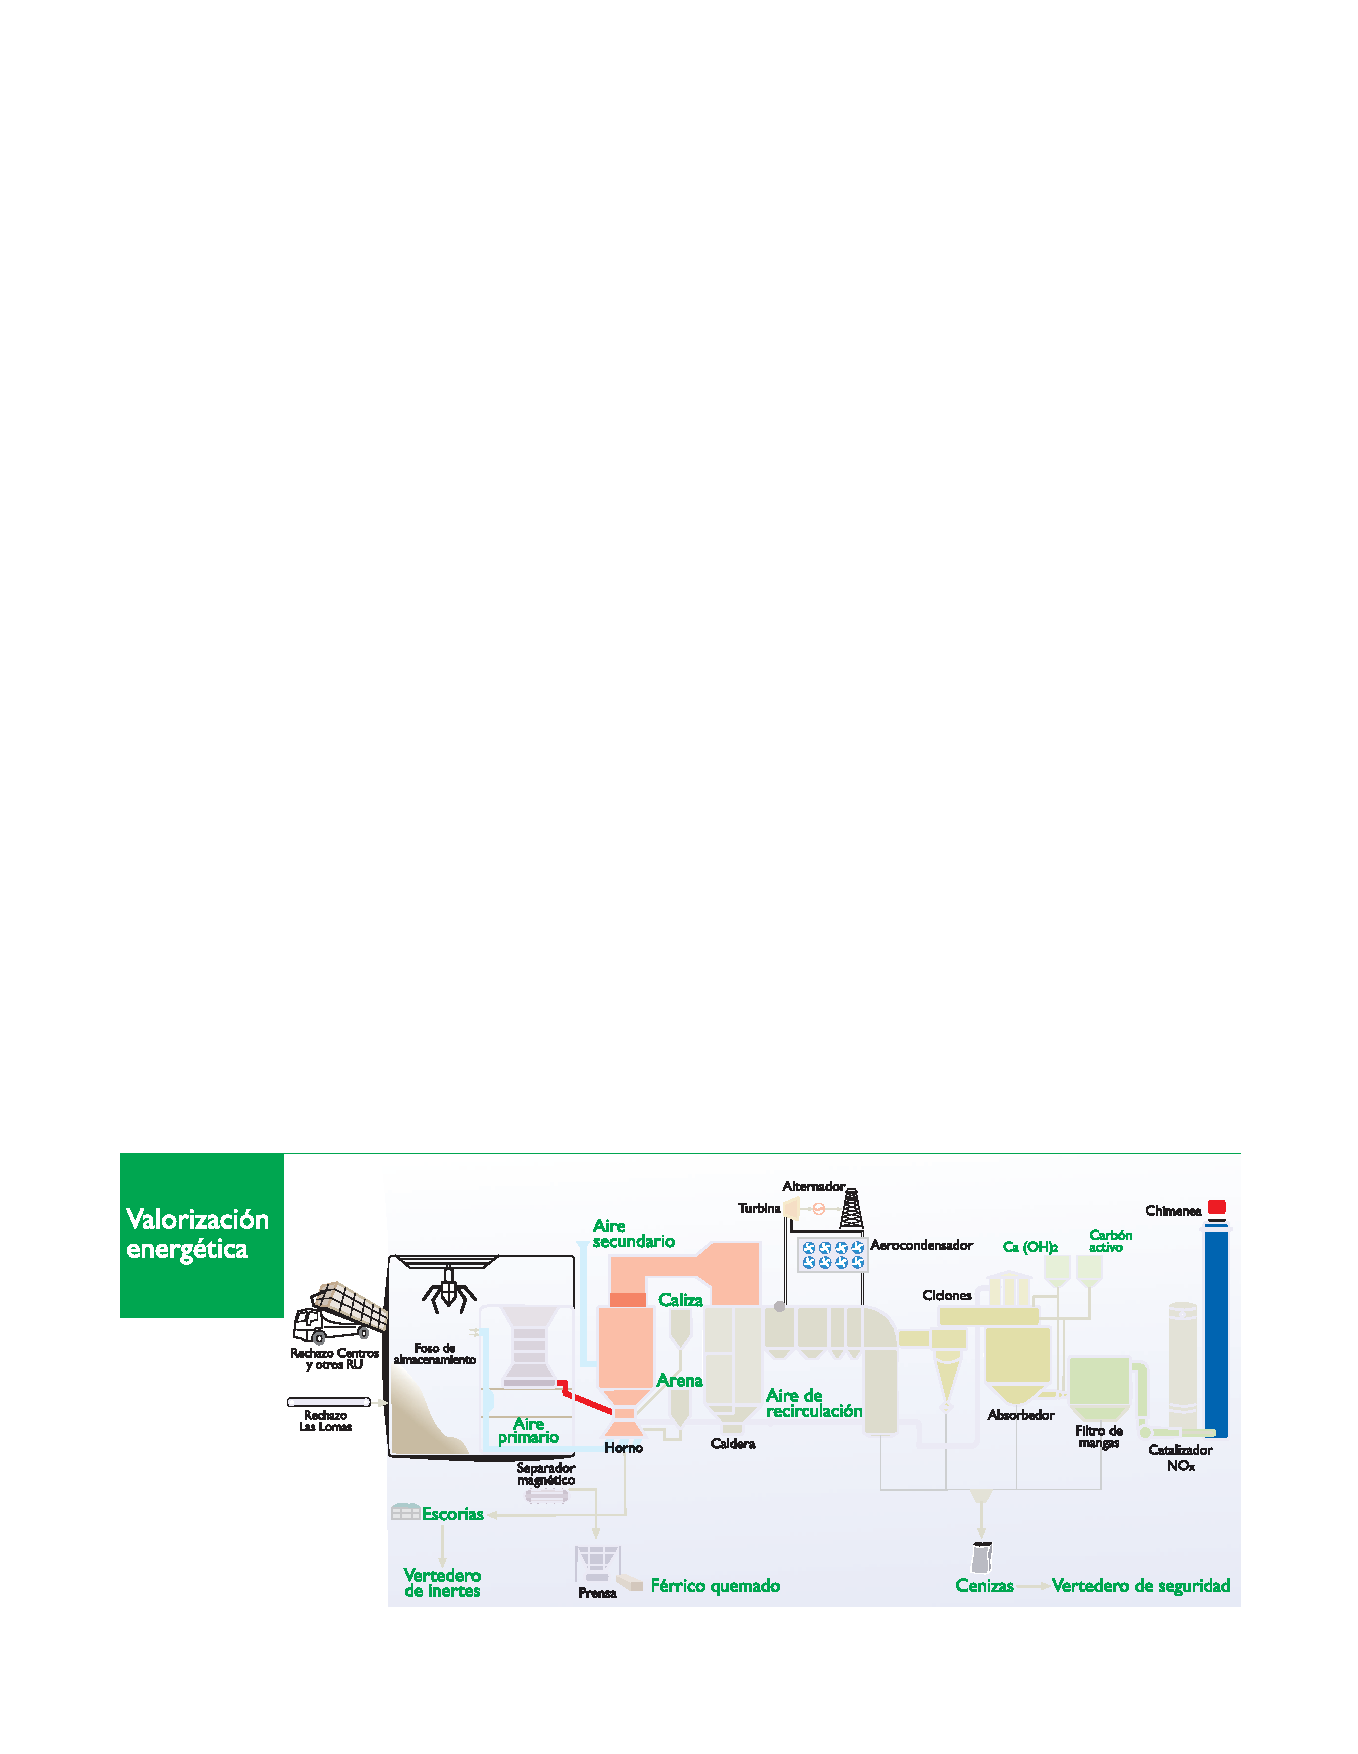
\includegraphics[height=5cm]{figuras/esquemasLomasValorizacion}
	\caption{Planta de valorización energética del Centro Las Lomas del Parque Tecnológico de Valdemingómez, donde se aprovecha los gases a alta temperatura para producir vapor de agua en la caldera para mover unas turbinas conectadas a generadores para producir electricidad. \textit{Fuente: Ayuntamiento de Madrid}}
	\label{fig:esquemaslomasvalorizacion}
\end{figure}
La principal desventaja de estos sistemas son el uso de partes móviles que tienen que estar en constante mantenimiento por desgaste, el uso de fluidos que complica el control del sistema. Otra desventaja de estos sistemas es que suelen requerir un tamaño mínimo a partir del cual pasan a ser rentables, con lo cual se reduce el en número de aplicaciones donde pueden ser utilizados. Sin embargo, los dispositivos de estado sólido (\acrshort{teg}, \acrshort{tic} y \acrshort{tpv}) son escalables, pudiendo encontrar más aplicaciones donde ser utilizados (a nivel residencial, en aplicaciones espaciales, automoción, etc.).\\

% Termo Electrico
Los \acrshort{teg} son dispositivos que convierten la energía térmica en electricidad y viceversa, que están compuestos por dos materiales con coeficientes Seebeck opuestos unidos en sus extremos \cite{tegDef1}. Al aplicarse una diferencia de temperatura entre ambas uniones se genera una diferencia de potencial, conocido esto como efecto Seebeck. Los materiales que se utilizan para estos dispositivos tienen unas conductividades térmicas bajas, para disminuir las pérdidas por conducción de calor. Para aumentar la potencia de los \acrshort{teg} se aumenta la diferencia de los coeficientes Seebeck porque cuanto mayor sea esta diferencia, mayor será la tensión y la potencia de salida, como se pueden observar en las ecuaciones de \cite{tegDef1}.\\

La eficiencia de los \acrshort{teg} es alrededor del 5\% \cite{TEG5efficiency}, aunque hasta el momento la eficiencia ha llegado como máximo hasta aproximadamente 15\% \cite{TEG15efficiency}, lo cual sigue siendo demasiado baja. Aún con bajas eficiencias los \acrshort{teg} se utilizan para aplicaciones espaciales, recuperación de calor en el transporte,entre otros.\\


% Termoiónico
Otro sistema de obtención de electricidad de una fuente de calor es la generación termoiónica, que mediante la emisión termoiónica se produce un flujo de electrones entre el emisor metálico a alta temperatura y un receptor a menor temperatura, separados por el vacío. Al aumentar la temperatura del emisor, los electrones libres se excitan hasta tal punto que la energía es lo suficientemente grande como para que se desprendan del material, la densidad de corriente está determinada por la ley de Richardson, donde $J=A\cdot T^2\cdot e^{\frac{-W}{k\cdot T}}$, siendo \textit{J} la densidad de corriente, \textit{A} la constante de Richardson, \textit{W} la función de trabajo del metal, \textit{k} la constante de Boltzman y \textit{T} la temperatura en Kelvin.\\

% Termofotovoltaico
Un generador que se puede combinar con el \acrshort{tic}, es un generador \acrshort{tpv} que transforman la radiación electromagnética producida por el emisor a alta temperatura para ser capturada por el receptor, que es una célula fotovoltaica (\acrshort{pv}). Los emisores de las \acrshort{tpv} no tienen que estar a unas temperaturas tan altas como los \acrshort{tic}, ya que no necesita que se desprendan los electrones. Ambos dispositivos presentan el mismo problema de pérdidas de electrones o fotones por los bordes del convertidor y para disminuir esto se disminuye la separación entre el emisor y el receptor. Cuando las distancias se vuelven nanométricas aumenta la transferencias de fotones por la transferencia de radiación evanescente y/o electrones por la eliminación del efecto de carga de espacio, generando una mayor potencia eléctrica porque la potencia radiada aumenta con respecto a la proporcionada por la ley de Planck, conocido como ``efecto de campo cercano''.\\

La eficiencia de las células \acrshort{tpv} han aumentado con el tiempo hasta llegar aproximadamente a un 40\% con una célula de dos uniones con materiales de ancho de banda (\acrshort{bg}) entre 1 y 1.4 eV, utilizando un reflector trasero que devuelve la radiación de menor energía al \acrshort{bg} directa al emisor, pero solo llegando a obtener una densidad de potencia de 2.39 $W{cm}^{-2}$ \cite{ThermalConductivity_SiO2_2018}. Se pueden obtener potencias eléctricas mayores mediante el uso del efecto de campo cercano.\\

Los dispositivos que aprovechan los efectos de campo cercano presentan la dificultad de mantener de manera constante las distancias de separación nanométricas a lo largo de grandes superficies (relativo a la distancia de separación), los dispositivos de campo cercano estudiados hasta la fecha presentan áreas muy pequeñas $<0.3 \ mm^2$ \cite{inoue_one-chip_2019_0_3mm2}. Para poder fabricar dispositivos TPV que aprovechan los efectos de campo cercano con un área considerable de $\sim 1 \ cm^2$, se requiere el uso nano-espaciadores. Por ejemplo, en \cite{doi:MicroGapTPV} usan espaciadores de $1\mu m$ de dióxido de silicio (\gls{sio2}) y se observó que al disminuir la distancia de separación la corriente de cortocircuito aumenta.


\section{Objetivos}
El objetivo de este estudio es diseñar y simular pilares de dimensiones nanométricas para el aprovechamiento del efecto de campo cercano en un convertidor \acrshort{tpv}, así como determinar la viabilidad de este sistema. 
\begin{itemize}
	\item Modelar un nano-espaciador dentro de los rangos permitidos de los parámetros de los programas de simulación y modelado 3D.
	\item Ensamblar los sistemas TPV para diferentes alturas del nano-espaciador para las simulaciones.
	\item Simular la transferencia de calor por conducción a través de un nano-espaciador de $SiO_2$ de un sistema TPV para diferentes alturas del nano-espaciador, diferentes materiales de emisor y diferentes resistencias de contacto entre emisor y el nano-espaciador.
	\item Simular la transferencia de calor radiada entre el emisor y la célula para diferentes materiales del emisor y para varias distancias de separación, teniendo en cuenta los efectos de campo cercano en la radiación.
	\item Determinar entre los casos estudiados cuales pueden dar lugar a sistemas de TPV de campo cercano viables.
\end{itemize}

%%% NECESARIO?
\section{Estructura del documento}

A continuación y para facilitar la lectura del documento, se detalla el contenido de cada capítulo.

\begin{itemize}
\item En el \textbf{capítulo 1} se realiza una introducción del trabajo con la respectiva motivación y objetivos.
\item En el \textbf{capítulo 2} se desarrolla el estado de arte, definiendo los apartados más importantes y resaltando las investigaciones con mayor relevancia.
\item En el \textbf{capítulo 3} se exponen las herramientas y materiales utilizados, así como los criterios de selección.
\item En el \textbf{capítulo 4} se mencionan los métodos seguidos y los cálculos realizados para el desarrollo del trabajo.
\item En el \textbf{capítulo 5} se exponen los resultados obtenidos de las simulaciones.
\item En el \textbf{capítulo 6} se desarrolla la conclusión y se realiza planteamientos para futuros trabajos.
\end{itemize}
